\chapter{Исследовательская часть}

\section{Интерфейс приложения}

На рисунке~\ref{fig:interface} представлен интерфейс приложения.

\begin{figure}[h!]
	\centering{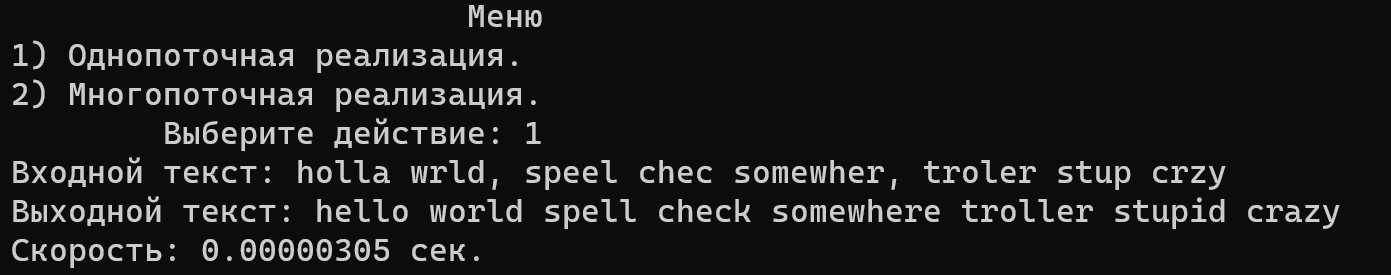
\includegraphics[scale=0.9]{photos/interface.png}}
	\caption{Интерфейс приложения}
	\label{fig:interface}
\end{figure}

\section{Технические характеристики}

Технические характеристики устройства:

\begin{itemize}
	\item операционная система --- Windows 11 Pro 64 -- разрядная система~\cite{windows};
	\item оперативная память --- 16 Гбайт;
	\item процессор --- 11th Gen Intel(R) Core(TM) i7-1165G7 с тактовой частотой 2.8 ГГц;
	\item количество ядер --- 4 физических и 8 логических ядер.
\end{itemize}

\section{Время выполнения реализаций алгоритмов}

На рисунке \ref{fig:graph1} приведено сравнение реализации последовательного и параллельного алгоритмов исправления орфографических ошибок в тексте. 
Время было найдено как среднее трех измерений.

\begin{figure}[ht!]
	\begin{center}
		\captionsetup{singlelinecheck = false, justification=centerfirst}
		\begin{tikzpicture}
			\begin{axis}[
				xlabel={Количество ядер},
				ylabel={Время в секундах},
				width = 0.95\textwidth,
				height=0.5\textheight,
				xmin=0, xmax=16,
				ymode=log, 
				legend pos=north west,
				legend style={font=\footnotesize},
				xmajorgrids=true,
				grid style=dashed,
				]
				
				\addplot[
				blue,
				semithick,
				mark = *,
				mark size = 3pt,
				thick,
				] file {graph/multi_thread.csv};
				
				\addplot[
				red,
				semithick,
				mark = x,
				] file {graph/single_thread.csv};
				
				\legend{
					Параллельный алгоритм,
					Последовательный алгоритм
				}
			\end{axis}
			
		\end{tikzpicture}
		\centering
		\caption{Сравнение времени работы реализаций алгоритмов}
		\label{fig:graph1}
	\end{center}
\end{figure}
\clearpage

\section*{Вывод}

В ходе сравнения параллельного и последовательного алгоритмов исправления ошибок в тексте выявлено, что при увеличении числа потоков до 4 производительность параллельной реализации значительно превосходит последовательную. 
Однако, при дальнейшем увеличении числа потоков до 8 наблюдается некоторое снижение эффективности из - за увеличения накладных расходов на управление потоками. 
Несмотря на это, алгоритм с 8 потоками остается более быстрым, чем последовательная реализация.

При использовании 16 и более потоков параллельная реализация проигрывает последовательной. 
Это связано с появлением проблемы конкуренции за ресурсы процессора, созданием большого числа потоков и увеличением объема обслуживаемой очереди, что в итоге снижает общую производительность.